\begin{appendices}
  \section{Cost Tables} \label{app:cost}
  \jules{In table \ref{table:r0} and \ref{table:r2}, external sorts also include spilling and reading back from disk in between the two sorts.}
  
\begin{table*}[]
\centering
\caption{TAAT plan cost table}
\label{table:r0}
\begin{tabular}{|c|c|c|c|}
\hline
Costs & Scenario 1 & Scenario 2 & Scenario 3 \\ \hline

0A: $\sigma(R)$  &  
 $\begin{aligned} & |E| Scan^{index} & \text{if } f_s \leqslant V(c_r,F) \\ & |E| Scan^{Sequential} & \text{else}\end{aligned}$ & & \\ \hline

0B: $F'[], \sigma(R)$ &  $|E| (n-1 \text{ joins})$      &            &            \\ \hline

0C: $\tau(\gamma_{inner}([])), F$    & 
$\begin{aligned} & 0 & \text{if }  \frac{|F|}{V(c_r,F)} \leqslant M f_s \\ & |E|(2 \text{ external sorts}) & \text{else}\end{aligned}$   & 
&
\\ \hline
\end{tabular}
\end{table*}

\begin{table*}[]
\centering
\caption{NSAAT plan cost table}
\label{table:r2}
\begin{tabular}{|c|c|c|c|}
\hline
Costs & Scenario 1 & Scenario 2 & Scenario 3 \\ \hline

2A: $E \rightarrow T$      &    \text{insignificant}        &            &            \\ \hline

2B: $\delta(\pi_{c_e}(T))$      &     \text{insignificant}       &            &            \\ \hline
      
2C: $\innerjoin([,R]), \delta(\pi_{c_e}(T))$ & 
$\begin{aligned} & Join^{right\_index}_{c_e = c_r}(\delta(\pi_{c_e}(T)),R) & \text{if } f_s \leqslant V(c_r,F) \\ & Join^{memory\_hash}_{c_e = c_r}(\delta(\pi_{c_e}(T)),R) & \text{else} \end{aligned}$ &
      &              \\ \hline

2D: $F'([]), \innerjoin(\dots)$ &    n-1 \text{joins}        &            &            \\ \hline

2E: $\chi(\gamma_{inner}([]), rf(F,T)$ & 
$\begin{aligned} & 0 & \text{if }  \frac{V(c_e,E)|F|}{V(c_r,F)} \leqslant M f_s \\ & 2 \text{ external sorts} & \text{else}\end{aligned}$ &            &            \\ \hline

2F: $\gamma_{\texttt{NEST}}([]), \chi(\dots)$      &  \text{insignificant}       &            &            \\ \hline

2G: $\leftouterjoin([T,])$      &     \text{insignificant}       &            &            \\ \hline
\end{tabular}
\end{table*}


\begin{table*}[]
\centering
\caption{DSAAT plan cost table}
\label{table:r4}
\begin{tabular}{|c|c|c|c|}
\hline
Costs & Scenario 1 & Scenario 2 & Scenario 3 \\ \hline
  4A: $F$    &     $n-1$ joins       &            &            \\ \hline
  
  4B: $\leftouterjoin([E,]),F$    &
  $\begin{aligned} & Join^{right\_index}_{c_e = c_r}(E,F) & \text{if } f_s \leqslant V(c_r,F)  \\ & & \text{ and $F$ is a relation} \\ & Join^{memory\_hash}_{c_e = c_r}(E,F) & \text{else} \end{aligned}$
   &            &            \\ \hline
 4C:  $\chi(\gamma_{inner}([]), \leftouterjoin(\dots) $    &  
  $\begin{aligned} & 0 & \text{if }  \frac{|E||F|}{V(c_r,F)} \leqslant M f_s \\ & 2 \text{ external sorts} & \text{else}\end{aligned}$   &            &           \\ \hline
  4D: $\gamma_{\texttt{NEST}}([]), \chi(\dots)$      &      \text{insignificant}    &            &            \\ \hline
\end{tabular}
\end{table*}

\eat{
\begin{table*}
\centering
\caption{Scenario 1 Total Costs using AsterixDB architecture}
\label{table:scenario1}
\begin{tabular}{|c|C{4.5cm}|C{4.5cm}|C{4.5cm}|}
\hline
 & $V(c,F) \geqslant f_s$ & $f_s \geqslant V(c_r,F) \geqslant  \frac{|F|}{M f_s}$ & $ \frac{|F|}{M f_s} \geqslant V(c,F)$ \\ \hline

$cost(R_0)$ 
& $|E| (\frac{|F|}{V(c,F)} + cost(F')) $
& ? % $|E|(\frac{|F|}{V(c,F)} + 2 \frac{|F|}{V(c,F)f_s} + 5 \frac{V(g,F)}{f_s})$
& $|E| (\frac{ F}{f_s} + 2 \frac{|F|}{V(c,F)f_s} + 5 \frac{V(g,F)}{f_s} + cost(F'))$ \\ \hline

$cost(R_2)$
& $ \frac{V(c,E)|F|}{V(c,F)} + cost(F') $
& ? % $\frac{|F|V(c,E)}{V(c,F)}+ \frac{|F|V(c,E)}{V(c,F)f_s} + 2\frac{|F|V(c,E)}{V(c,F)f_s} + 5\frac{V(g,F)V(c,E)}{f_s}$
& $\frac{F}{f_s} + \frac{V(c,E)|F|}{V(c,F)} + 2\frac{|F|V(c,E)}{V(c,F)f_s} + 5 \frac{V(g,F)V(c,E)}{f_s} + cost(F') $  \\ \hline 

$cost(R_4)$ & $\frac{|E||F|}{V(c,F)} + cost(F)$ 
& ? % $\frac{|E||F|}{V(c,F)} + \frac{|E||F|}{V(c,F)f_s} + 2 \frac{|E||F|}{V(c,F)f_s}  + 5 \frac{|E|V(g,F)}{f_s}$
& $\frac{F}{f_s} + \frac{|E||F|}{V(c,F)f_s} + 2 \frac{|E||F|}{f_s V(c,F)} + 5 \frac{|E|.V(g,F)}{f_s} + cost(F)$ \\ \hline

Winner
& $cost(R_2) < cost(R_4) < cost(R_0)$
& ?
& $cost(R_2) < cost(R_4) < cost(R_0)$ \\ \hline
\end{tabular}
\end{table*}
}

\begin{figure*}
\centering
\caption{Scenario 1 \label{fig:scenario1}}
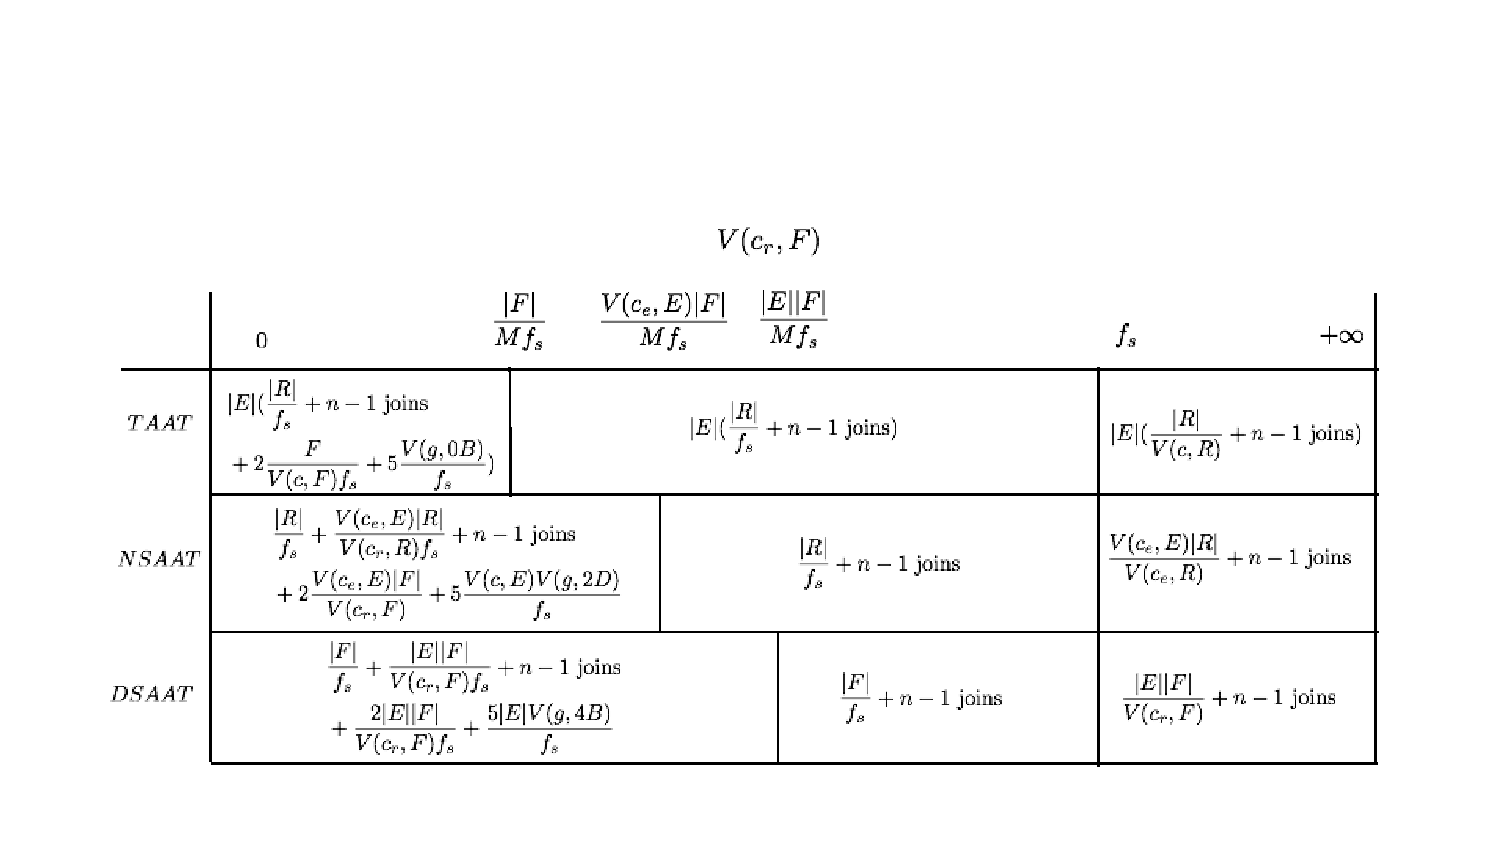
\includegraphics[width=15cm]{images/Scenario1.pdf}
\end{figure*}
  
  
\section{Examples} \label{app:examples}
Here are provided the queries for the use cases given in section 2. Note that all queries are expressed using the SQL++ language developed at UCSD \cite{ong:2014aa}, although those queries would be typically written using an application-specific query language. 

\begin{figure}[h]
\label{fig:schema}
\centering
\caption{TPCx-BB Schema}
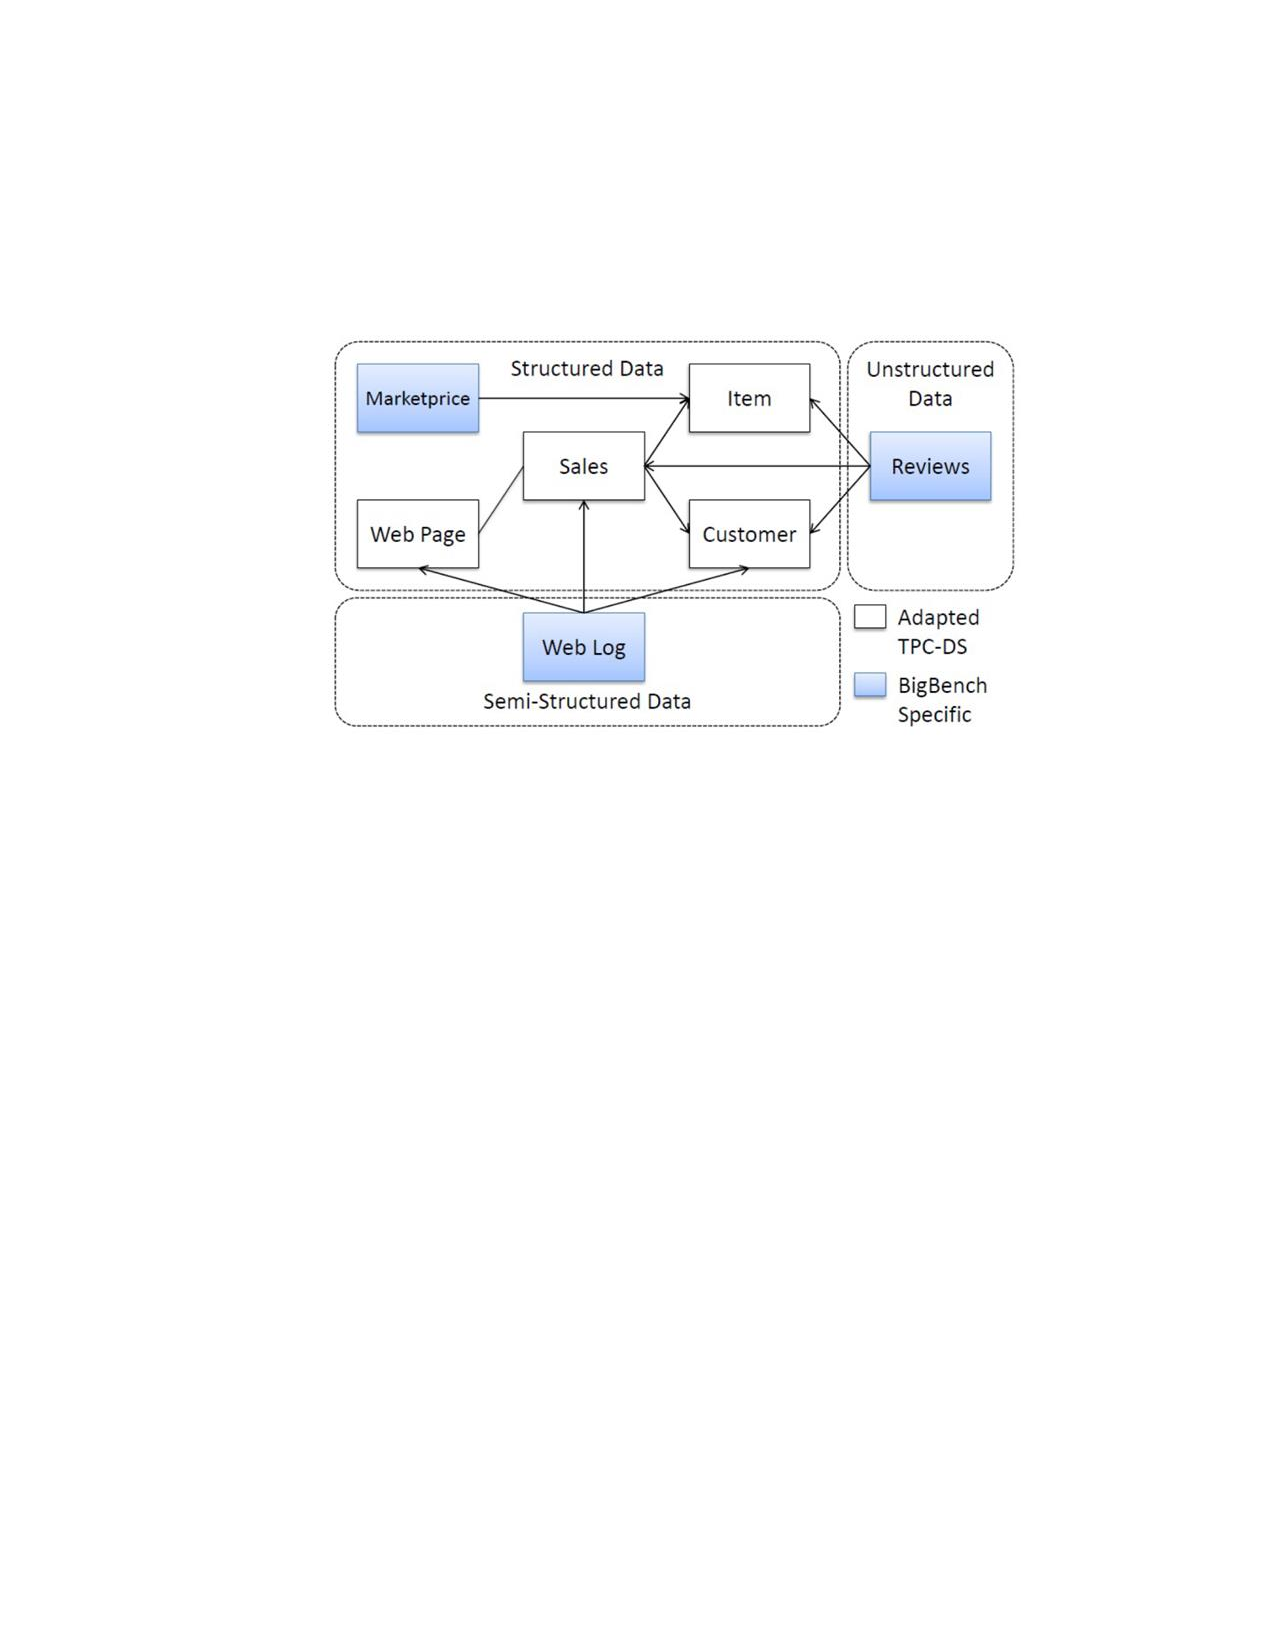
\includegraphics[width=\linewidth]{images/schema.pdf}
\end{figure}

Example \ref{list:query1} produces pre-aggregated hit-counts per minute and per hour for a webpage $Y$ on a day $X$. Example \ref{list:query2} produces this output for all distinct \{day,webpage\} pairs. Examples \ref{list:query1} and \ref{list:query2} are representative of scenarios $S3_S$ and $S3_L$, respectively.
\lstinputlisting[language=SQL,label={list:query1},caption={Operational Intelligence example, local}]{code/query1.sql}
\lstinputlisting[language=SQL,label={list:query2},caption={Operational Intelligence example, global}]{code/query2.sql}

Example \ref{list:query3} corresponds to the query 2 from the TPCx-BB benchmark. It finds the top 30 products that are mostly viewed together with a given list of products in an online store. Note that the order of products viewed does not matter, and "viewed together" relates to a web\_clickstreams \texttt{click\_session} of a known user with a session timeout of 60min.

\lstinputlisting[language=SQL,label={list:query3},caption={TPCx-BB Query 2}]{code/query3.sql}

Example \ref{list:query4} finds, for each clerk from a (small) set of selected clerks working in store $X$, the total price of the top $K$ orders made by that clerk.

\lstinputlisting[language=SQL,label={list:query4},caption={Top orders from the same clerk for selected orders}]{code/query4.sql}

\end{appendices}